\documentclass[../main]{subfiles}

\begin{document}
\subsection{Experimento 1}
Analizando cada intervalo de interés:
\begin{table}[H]
  \caption{Datos para calcular la velocidad instantánea}\label{tab:meanv}
  \begin{center}
    \begin{tabular}{lSS}
      \toprule
      \multicolumn{1}{c}{\textbf{Tramo}} &
      \multicolumn{1}{c}{$\Delta t$ ($\delta = \qty{0.13}{\s}$)} &
      \multicolumn{1}{c}{$\frac{\Delta x}{\Delta t}$ (\unit{\cm\per\second})}\\
      \midrule
      $AC$ & \num{9.28} & \num{2.14(4)}\\
      $AC_1$ & \num{4.66} & \num{3.20(10)}\\
      $AC_2$ & \num{2.78} & \num{3.60(19)}\\
      $AC_3$ & \num{1.23} & \num{3.98(46)}\\
      $CB$ & \num{3.84} & \num{5.21(19)}\\
      $CB_1$ & \num{2.95} & \num{5.08(24)}\\
      $CB_2$ & \num{2.09} & \num{4.78(32)}\\
      $CB_3$ & \num{1.11} & \num{4.59(58)}\\
      \bottomrule
    \end{tabular}
  \end{center}
\end{table}

Resumiendo lo anterior en un gráfico:
\begin{figure}[H]
  \begin{center}
    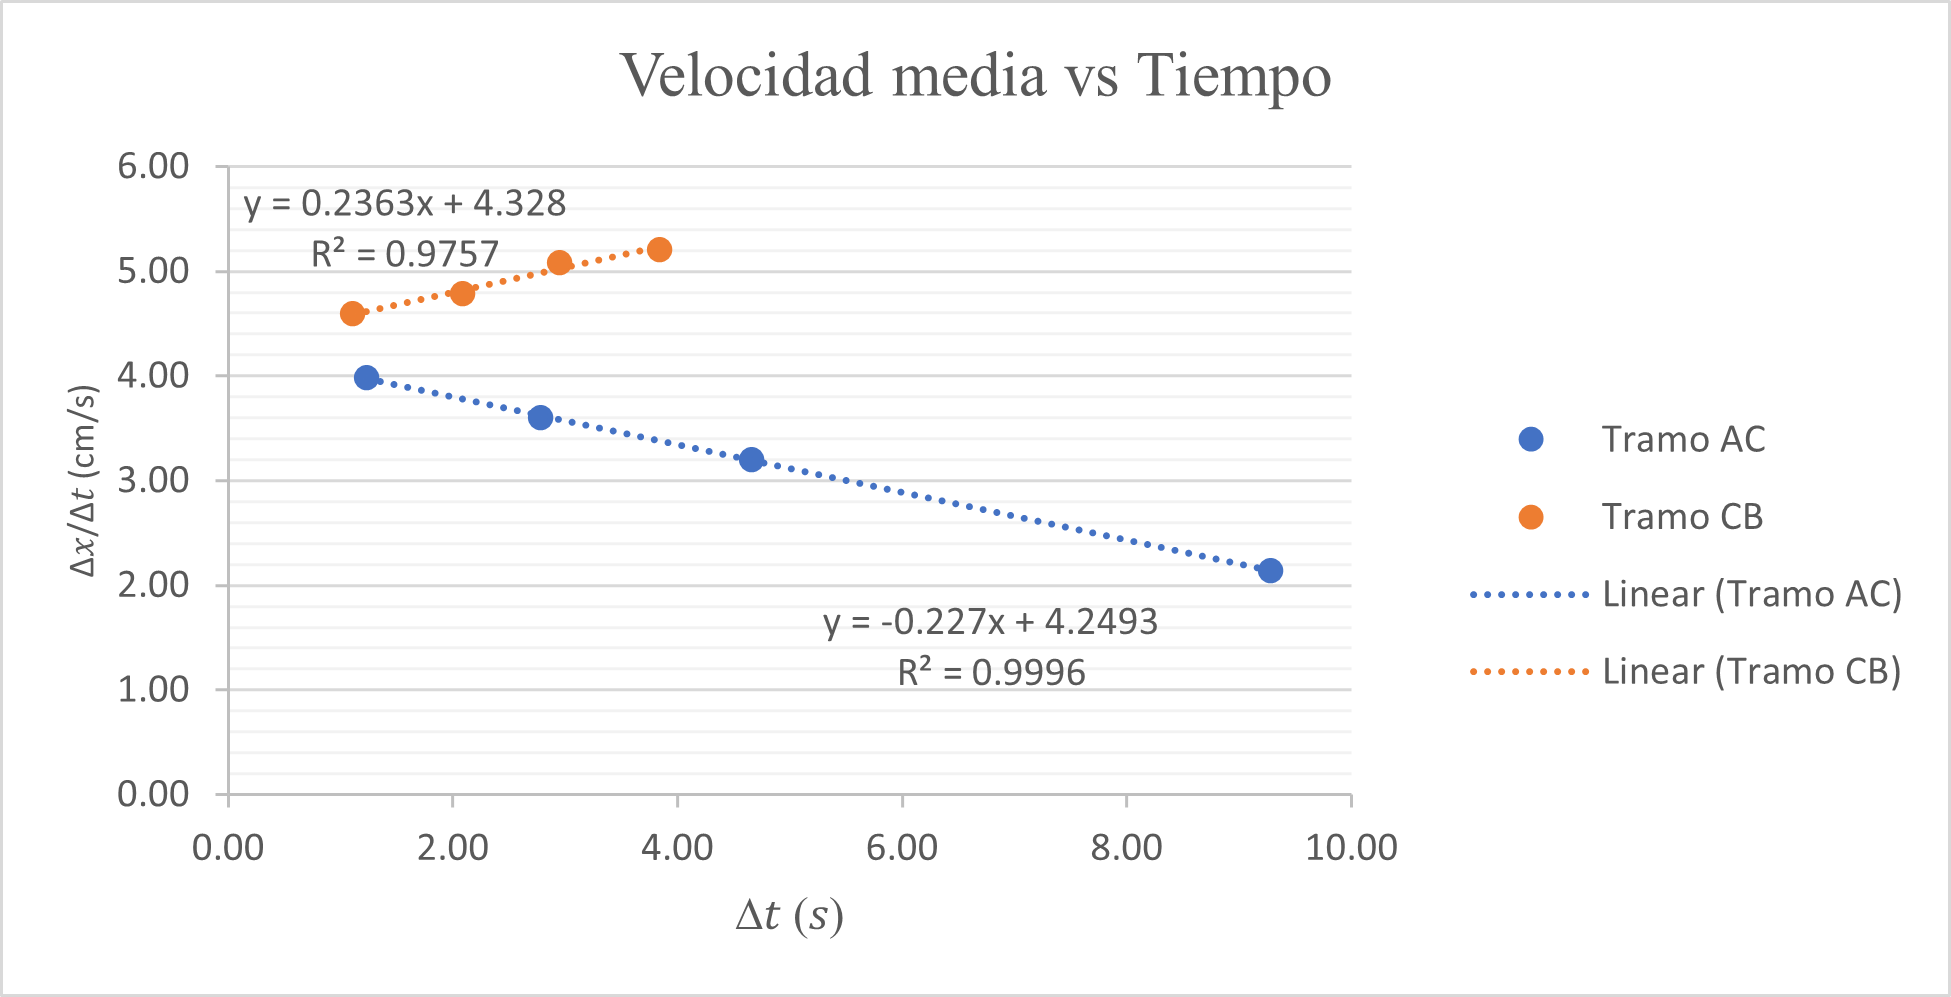
\includegraphics[width=0.65\textwidth]{res/vavg.png}
  \end{center}
  \caption{Velocidad media como función del tiempo}\label{fig:vavg}
\end{figure}

Visualizando las prolongaciones de ambos conjuntos:
\begin{figure}[H]
  \begin{center}
    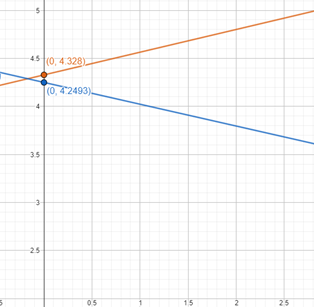
\includegraphics[width=0.35\textwidth]{res/compare.png}
  \end{center}
  \caption{Prolongación de las rectas de ambos tramos}\label{fig:compare}
\end{figure}

\subsection{Experimento 2}
Analizando cada intervalo de interés:
\begin{table}[H]
  \caption{Datos para calcular la aceleración instantánea}\label{tab:meanv2}
  \begin{center}
    \begin{tabular}{lSSS}
      \toprule
      \multicolumn{1}{c}{\textbf{Tramo}} &
      \multicolumn{1}{c}{$\Delta t$ ($\delta = \qty{0.13}{\s}$)} &
      \multicolumn{1}{c}{$t_i$ ($\delta = \qty{0.13}{\s}$)} &
      \multicolumn{1}{c}{$v_i$ (\unit{\metre\per\second})}\\
      \midrule
      $AA_1$ & \num{6.92} & \num{3.46} & \num{1.45(3)}\\
      $AA_2$ & \num{8.86} & \num{7.89} & \num{2.25(4)}\\
      $AA_3$ & \num{11.47} & \num{10.17} & \num{2.598(34)}\\
      $AA_4$ & \num{12.43} & \num{11.95} & \num{3.202(38)}\\
      \bottomrule
    \end{tabular}
  \end{center}
\end{table}

Resumiendo lo anterior en un gráfico:
\begin{figure}[H]
  \begin{center}
    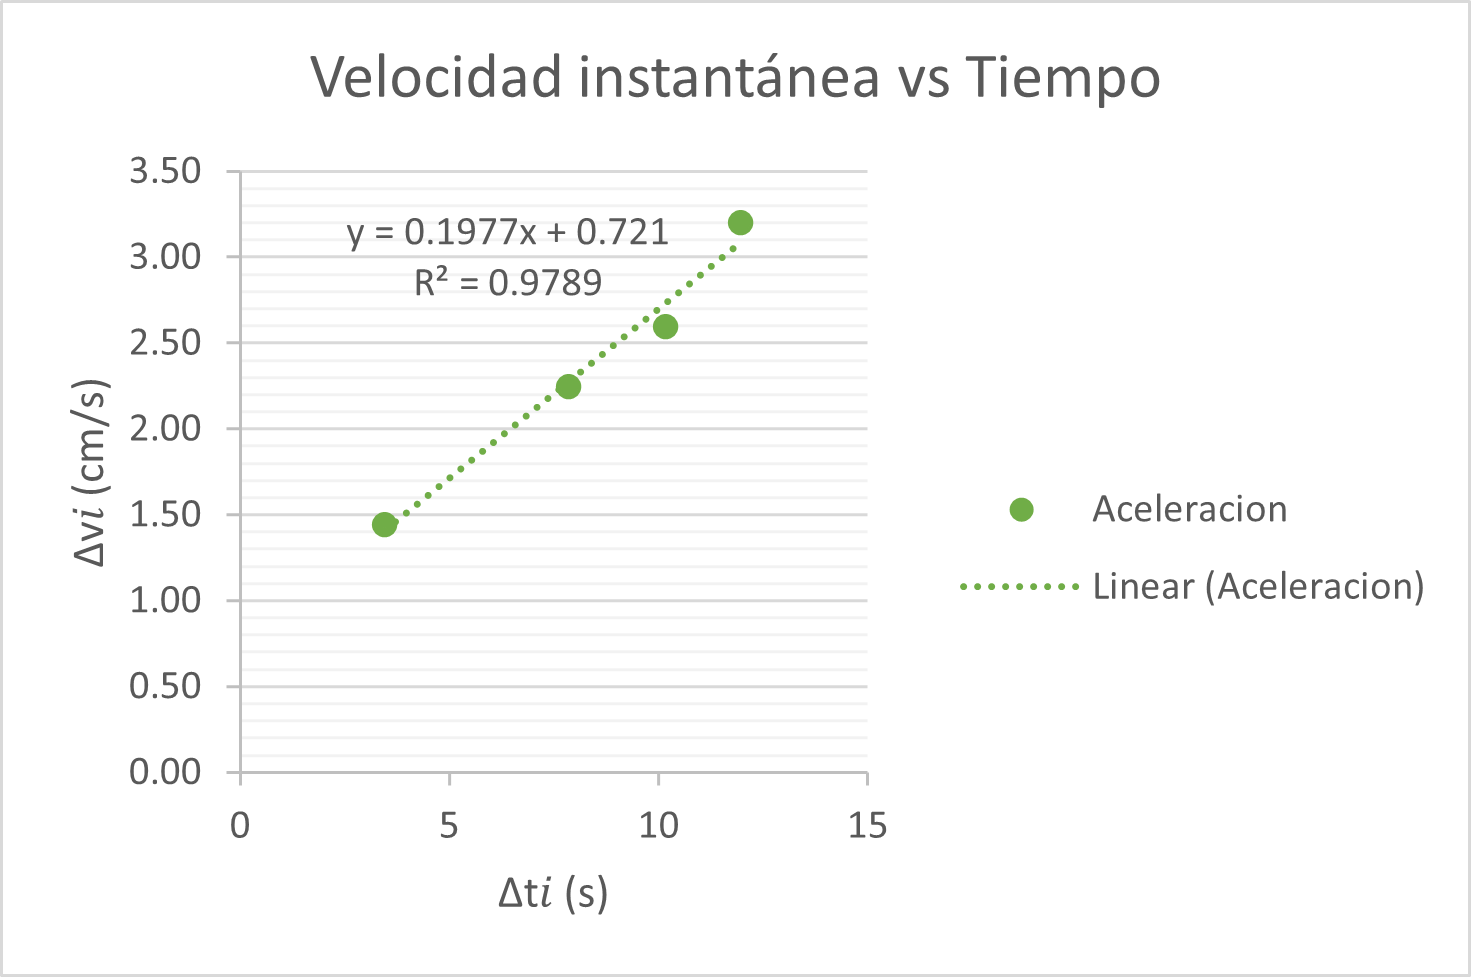
\includegraphics[width=0.65\textwidth]{res/vins.png}
  \end{center}
  \caption{Velocidad instantánea como función del tiempo}\label{fig:vins}
\end{figure}
\end{document}
